\documentclass[12pt]{article}
\usepackage{frExamplee}
\usepackage{booktabs}       % professional-quality tables
\usepackage{amsfonts}       % blackboard math symbols
\usepackage{amsmath}
\usepackage{amssymb}
\usepackage{graphicx}
\usepackage{csquotes}
\usepackage[backend=biber, style=ieee,]{biblatex}
\usepackage{setspace}
\usepackage[usenames, dvipsnames]{xcolor}
\usepackage{xspace}
\usepackage{caption}
\usepackage{subcaption}
\usepackage{multirow}
\usepackage{float}
\usepackage{wrapfig}
\usepackage{placeins}
\usepackage{algpseudocode}
\usepackage{algorithm}
\usepackage{algorithmicx}
\usepackage{hyperref}
% \doublespacing
\usepackage{setspace}
\setstretch{1.4}
\usepackage{fancyhdr} 
\fancyhf{}
\cfoot{\thepage}
\pagestyle{fancy}
\renewcommand{\headrulewidth}{0pt}%

\addbibresource{FRtemplates/frExampleRefs.bib}

\title{Thermodynamic State Properties in Gaseous Systems}

\author{
Tony Wang \\
1009027447\\
Sept 20 3-6PM Group 1
\And
Aiqi Zhang\\
1009253521\\
Sept 20 3-6PM Group 1
\And
Cordelia Woo\\
1009271440\\
Sept 20 3-6PM Group 1
}

\begin{document}

\maketitle

\begin{abstract}
Thermodynamic concepts, such as pressure and temperature, formed the foundation of many scientific and engineering disciplines, influencing the efficiency and operational aspects of various systems ranging from engines to turbines. This report aims to explore the relationship between key state variables in thermodynamics the aid of the Ideal Gas Law. Through the exchange of matter and their thermodynamic interactions, this experiment studies interactions during different controlled equilibriums. Phenomenons observed were noted and discussed using foundational principles, and unknowns values were mathematically computed using experimental results.
\end{abstract}
% \fbox{$\displaystyle \scalemath{I=\frac{dq}{dt}}$}
\section*{Introduction}
This experiment implemented the Ideal Gas Law \autocite{chandra2016energy}, a cornerstone of thermodynamics, and sought to gain insights from its applications:

\begin{equation}
P V = mRT 
\end{equation}

Where $P$ symbolized the system's pressure, represented in $[psi]$ for this lab; $V$ depicted the volume encapsulated by the system in $[m^3]$; $R$ embodied the gas constant of air, $0.2870kJ\cdot kg^{-1}\cdot K^{-1}$ in this case and finally, $T$ designated the system's temperature in an absolute scale, $[K]$. 

Concurrently, this experiment emphasized the relevance of the law of conservation of mass, an inherent property of the universe stating that in chemical processes, while the form of matter could drastically change, the overall amount of mass remained unchanged. This principle provided a lens to examine the transformation of matter at a more microscopic level. 

The experimental objectives included determining the volume ratio between two tanks under specific initial and equilibrium conditions, analyzing the heat transfer transformation during the expansion processes, understanding the route-independence of state properties, verifying the initial mass and volume of the left chamber, and finally confirming the reliability of our data. 

Particular attention was paid to the calculation of uncertainties, where source uncertainties were either given or interpreted visually, and other uncertainties were propagated in accordance to:
\begin{equation}
    u(y)=\sqrt{\sum^n_{i=1}\left(\frac{\partial y}{\partial x_i}\right)^2 },\text{ where }y=y(x_1, x_2...x_n).
\end{equation}
This meticulous approach \autocite{lee2009comparative} ensured the utmost accuracy in our findings, providing more solid and reliable conclusions from the experiment.

\section*{Experimental Method}
\subsection*{Apparatus}
At each workstation, the primary apparatus comprised two air tanks, sensors, pipes, and valves to assess the thermodynamic state of the tanks under varying conditions. The diagram below illustrated the fundamental configuration of the workstation, highlighting the adjustable valves that would be used in the experiment.
\begin{figure}[t!]
\centering
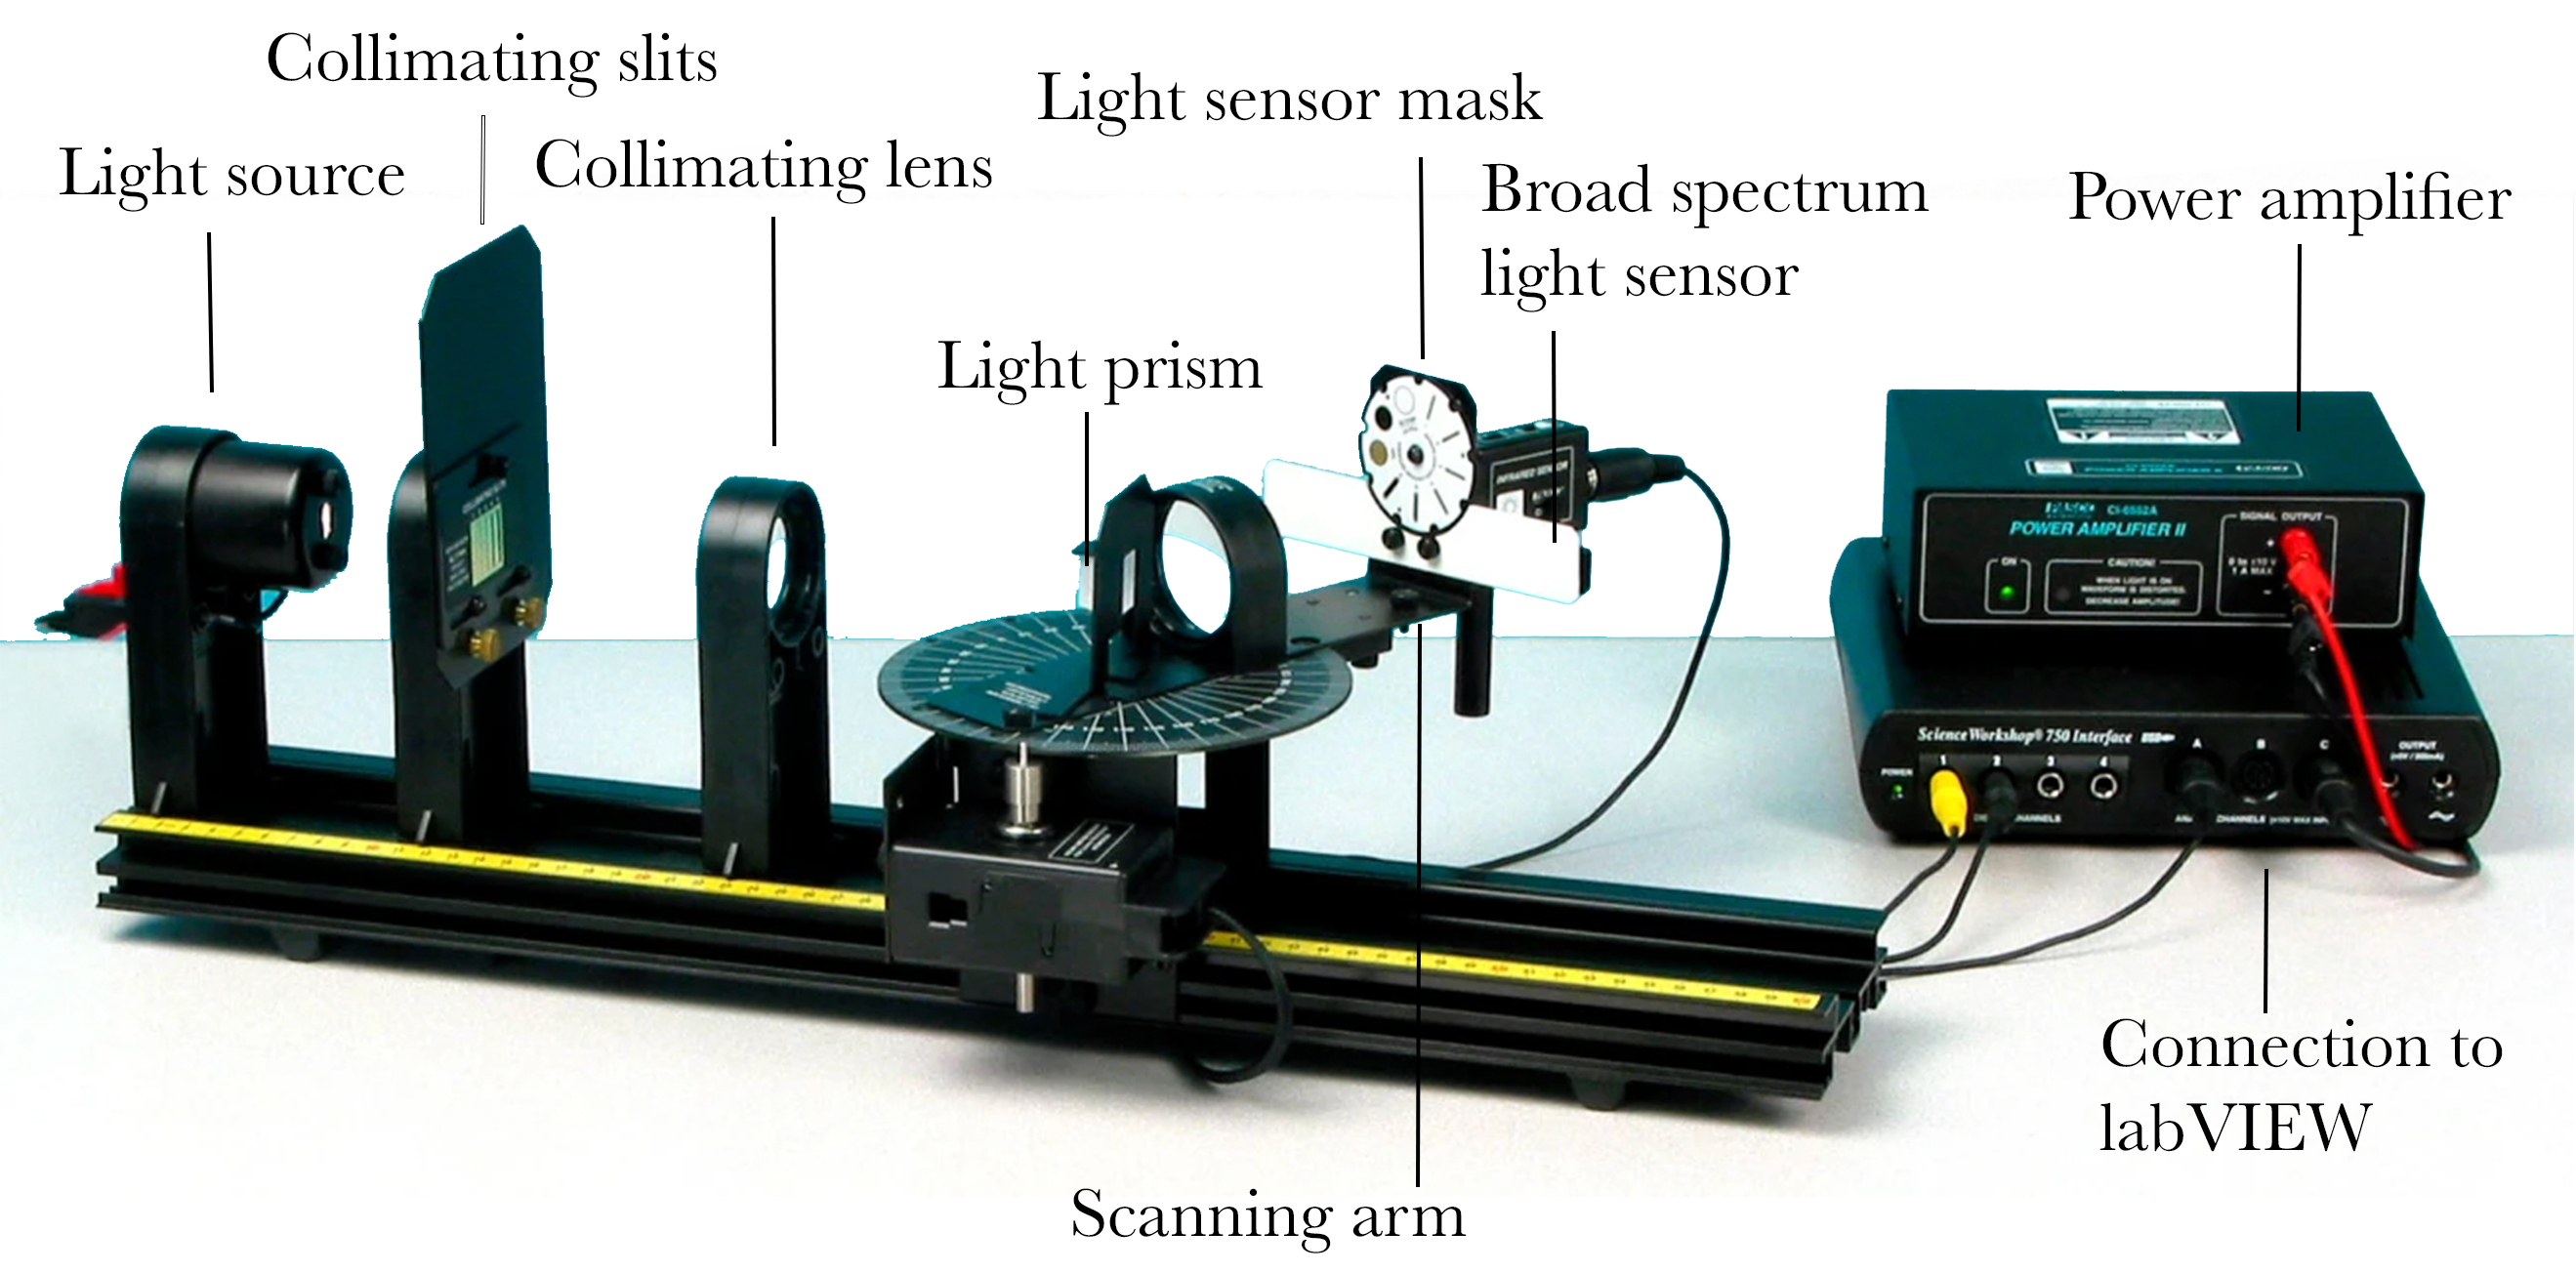
\includegraphics[width=0.7\linewidth]{figure/aparatus.png}
\caption{Drawing of experiment apparatus.}
\label{fig:aparatus}
\end{figure}
\begin{itemize}
    \item Tank: A separate space where the thermodynamic state of the gas could be controlled and experimented with.
    \item Yellow Valve: Controlled the flow path of the gas, if the valve was perpendicular to the pipe, it was in the closed position.
    \item Black Valve B1: Vented the gas out to the atmosphere when opened.
    \item Micrometer Needle Valve \& Small Ball Valve B2: Controlled the channel between the left tank and the right tank, the more the micrometer needle valve was opened (counterclockwise), the faster the gas was transferred.
    \item Pressure Gauge: Indicated the current air pressure within each tank.
    \item Air Valve: Connected with the external atmosphere and must be closed to ensure a separate space.
\end{itemize}
In addition to our setup in Fig. \ref{fig:aparatus}, a manometer was used to record the external atmosphere’s thermodynamic properties in the laboratory. The LabVIEW software would be employed for data recording and managing the workstation's electrical components. In the software, the Left/Center/Right Solenoids and flow speed would regulate air flow within the tanks, and the record/reset/save data buttons were designed for further data analysis. 

\subsection*{Procedure (Experiment I)}
The objective of part one was to confirm the path independency of thermodynamics state properties and to determine the volume ratio of the tanks. The basic idea was to expand air from pressurized tanks at two different rates, with uniform initial conditions, and then to record the thermodynamic state properties as the tanks reached thermal equilibrium.
\begin{enumerate}
    \item Initialize two tanks: 
    \begin{enumerate}
        \item Opened Valve A2 to pressurize the left tank to $40[psig]$ gauge pressure.
        \item Opened Valve A1 and A5 to vacuum the right tank to $-6[psig]$ gauge pressure.
    \end{enumerate}
    \item Method 1 - Using the Center Solenoid Valve: 
    \begin{enumerate}
        \item Opened the center solenoid valve.
        \item Allowed both tanks to achieve thermal equilibrium.
        \item Recorded the data for approximately 260 seconds.
    \end{enumerate}
    \item Method 2 - Using the Micrometer Needle Valve: 
    \begin{enumerate}
        \item Opened both the small ball valve B2 and the micrometer needle valve.
        \item Ensured the tanks maintained thermal equilibrium during the equalization process, aiming to approach the quasi-equilibrium process.
        \item Recorded the data for approximately 730 seconds.


    \end{enumerate}
\end{enumerate}

\subsection*{Procedure (Experiment II)}
The aim of Part Two was to determine the initial mass and volume of the left tank. Following a pressurization process, once the thermodynamic properties within the tank stabilized, the mass could be deduced from the area under the mass flow rate graph, and subsequently, the volume could be computed. 
\begin{enumerate}
    \item Opened Valve A2.
    \item Adjusted the flow rate to 50$\left[\frac{g}{min}\right]$.
    \item Pressurized the left tank to 40 [psi] gauge pressure. 
    \item Once the pressure and temperature stabilized, discharged the gas to the external environment.
\end{enumerate}

\section*{Results and Discussion}
\subsection*{Experiment I}
\begin{figure}[t!]
    \centering
    \subfloat[Comparison of two methods]{
        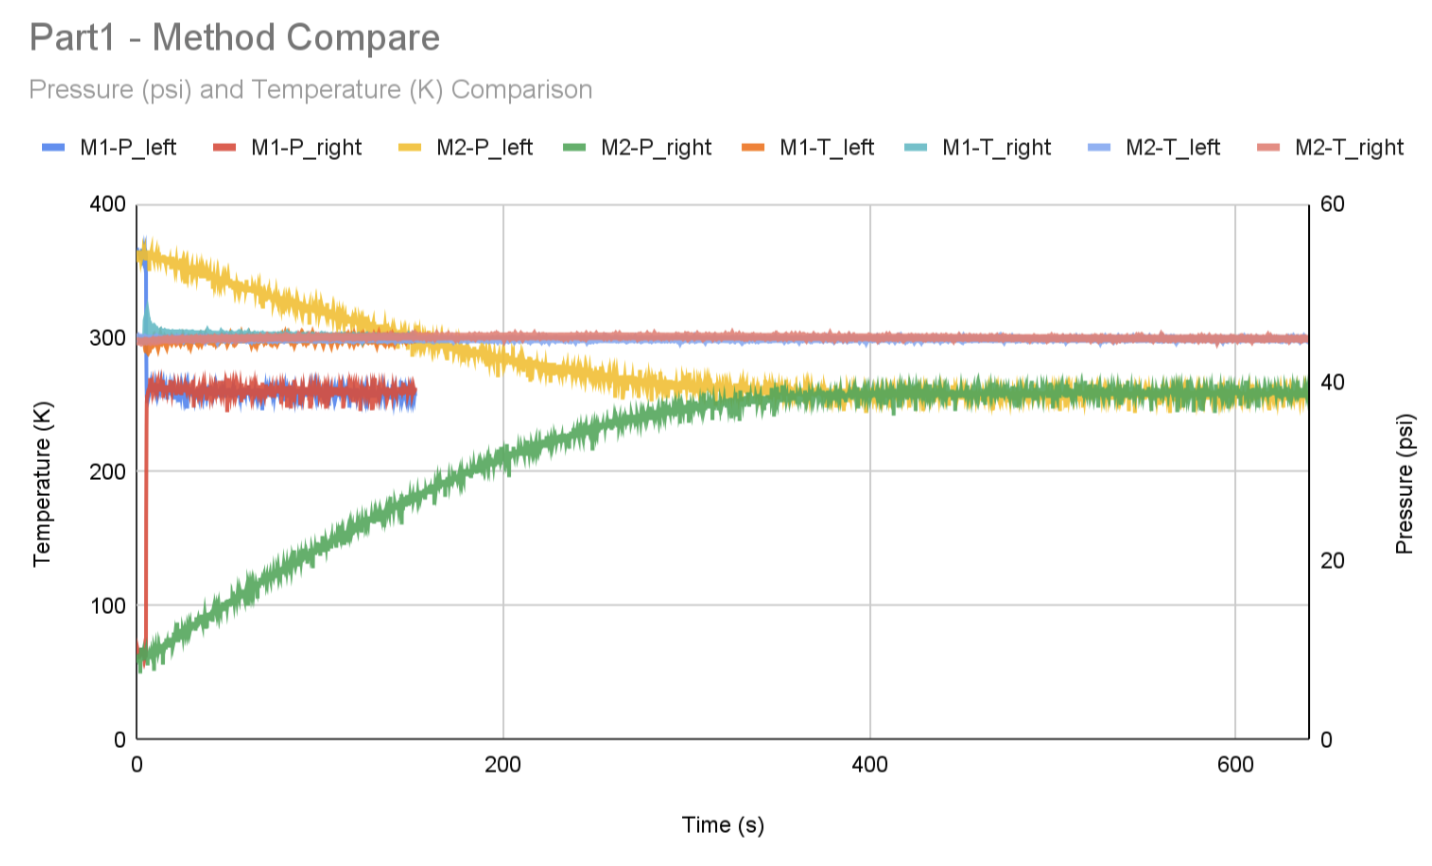
\includegraphics[width=0.7\columnwidth]{figure/method_compare.png}
        \label{fig:method_compare}
    }
    \hfill
    \subfloat[Method 1]{
        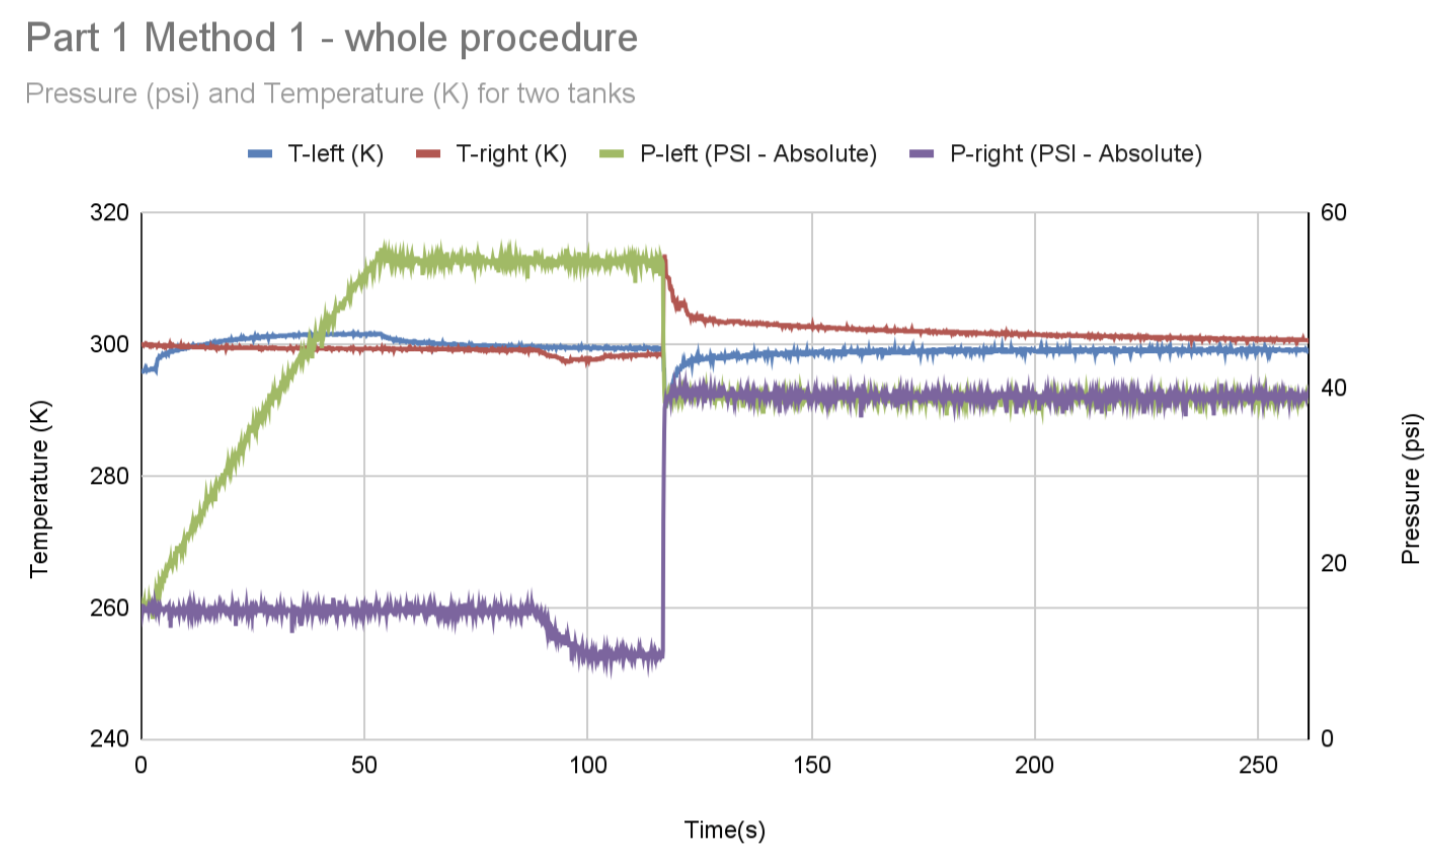
\includegraphics[width=0.49\columnwidth]{figure/p1m1.png}
        \label{fig:p1m1}
    }
    \hfill
    \subfloat[Method 2]{
        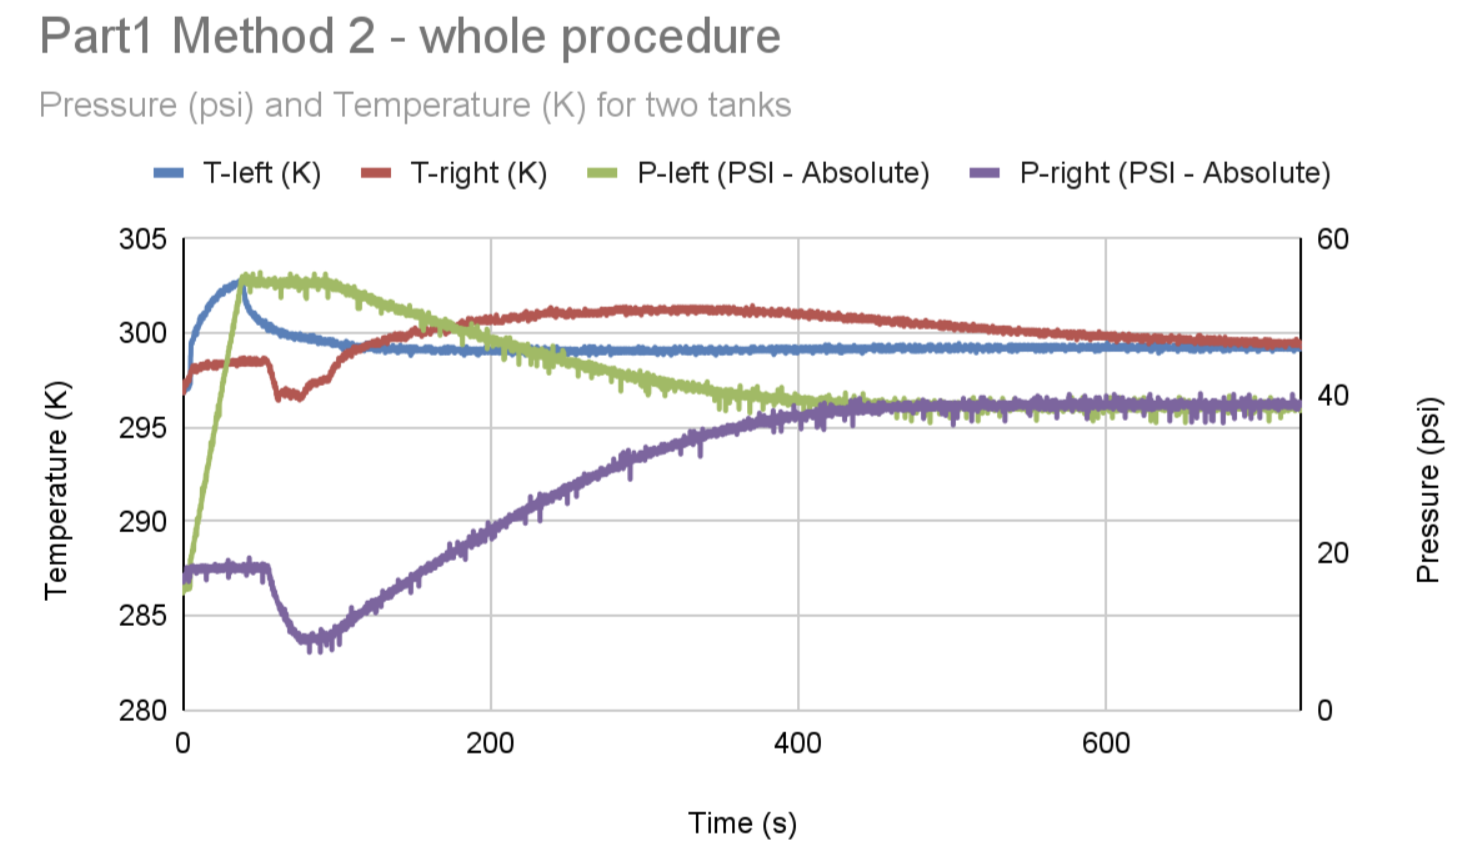
\includegraphics[width=0.46\columnwidth]{figure/p1m2.png}
        \label{fig:p1m2}
    }
    \caption{Plots of recorded data for experiment I.}
    \label{fig:graphs1}
\end{figure}
The thermodynamic states of the two tanks achieved identical equilibrium under the same initial conditions, as the properties converged to equal values at two distinct rates (Fig. \ref{fig:method_compare}). 
In method one (Fig. \ref{fig:p1m1}), using the center solenoid valve, the pressures of both tanks converged to a mutual value of $39\pm0.3[psig]$ (uncertainty interpreted visually from the maximum value spike of recorded data in linear regions) within $0.2[s]$ of the valve opening. At the same time, the temperatures of the tanks experienced a distinct divergence, peaking at a difference of $20.5[K]$. However, as time progressed, they finally converged to a uniform value of $299.9\pm0.2[K]$ in approximately $100[s]$.
In method two (Fig. \ref{fig:p1m2}) of using the micrometer needle valve, after the valve was opened, the pressures of the two tanks gradually converged to the same value of $38.7\pm0.3[psig]$ within an estimated time of $340\pm30[s]$ (uncertainty interpreted visually by estimating the interval where the two curves converge) after opening the valve. The convergence rate of the pressures was initially swift, decreasing gradually to zero. In contrast, the temperatures initially diverged slowly, with the maximum difference reaching $2.4[K]$ around $200[s]$ post-valve activation. Subsequently, they slowly converged to a value of $299.3\pm0.2[K]$ over $600[s]$.

\subsubsection*{Discussion}
\begin{itemize}
    \item The Ideal Gas Law and conservation of mass were used to determine the volume ratio:\\
    Since the gas worked with was assumed to behave ideally:
    \begin{equation}
        \begin{cases}
            P_{1i}V_1&=n_1RT_{1i}\\
            P_{2i}V_2&=n_2RT_{2i}
        \end{cases}
    \end{equation}
    Understanding that $n,\;R$ remained constant throughout:
    \begin{equation}
        \frac{P_{1i}V_1}{T_{1i}}+\frac{P_{2i}V_2}{T_{2i}}=\frac{P_fV_1}{T_f}+\frac{P_fV_2}{T_f}
    \end{equation}
    Which could be rearranged to get:
    \begin{equation}
        \frac{V_1}{V_2}={\frac{\frac{P_{f}}{T_{f}}-\frac{P_{2i}}{T_{2i}}}{\frac{P_{1i}}{T_{1i}}-\frac{P_{f}}{T_{f}}}}
    \end{equation}
    The initial condition in the calculation should be when the two tanks were in thermal equilibrium, having gauge pressures of $40[psig]$ and $-10[psig]$. The final state properties should be when both tanks achieved equilibrium. Plugging the numbers in the initial equilibrium and final equilibrium, calculations yielded a volume ratio of $1.78\pm0.08$ (uncertainty determined by propagating $u(P)=0.3$ and $u(T)=0.2$).
    % \begin{align}
    %     \text{Initially, }P_{1i}V_1&=n_1RT_{1i}\\\\
    %     \text{and }P_{2i}V_2&=n_2RT_{2i}.\\
    %     \text{And in the end, }P_f(V_1+V_2)&=(n_1+n_2)RT_f.\\
    %     \text{With constant mass, }n, R &= c\\
    %     \implies\frac{P_{1i}V_1}{T_{1i}}+\frac{P_{2i}V_2}{T_{2i}}&=\frac{P_fV_1}{T_f}+\frac{P_fV_2}{T_f}\\
    %     V_1\left(\frac{P_{1i}}{T_{1i}}-\frac{P_{f}}{T_{f}}\right)&=V_2\left(\frac{P_{f}}{T_{f}}-\frac{P_{2i}}{T_{2i}}\right)\\
    %     \frac{V_1}{V_2}&={\frac{\frac{P_{1i}}{T_{1i}}-\frac{P_{f}}{T_{f}}}{\frac{P_{f}}{T_{f}}-\frac{P_{2i}}{T_{2i}}}}\\
    %     \frac{V_1}{V_2}&={\frac{\frac{P_{1i}}{T_{1i}}-\frac{P_{f}}{T_{f}}}{\frac{P_{f}}{T_{f}}-\frac{P_{2i}}{T_{2i}}}}=1.85\pm0.02
    % \end{align}
    \item Heat transfer between tanks and surroundings: \\
    Heat transfer is a mechanism that occurs due to the temperature difference, described as “conveying energy and entropy” from a higher to a lower temperature \autocite{heat-transfer-britannica}. During Part 1, the temperature of the left chamber rose until the pressure reached 40 psi. After the valve was closed, the tank gradually achieved thermodynamic equilibrium, characterized by constant properties, until the opening of the valve. As the pressure increases in the left tank, the work done of pressurization will increase the internal energy of the gas, thus resulting in a higher temperature. Similarly, the temperature of the right chamber decreased along with the pressure and remained constant until the system was altered. The tank’s vacuum caused negative work, affecting a reduction in internal energy and a temperature drop.
    After the valve was opened, the temperature of both tanks exhibited a divergence and eventually converged to a constant at two distinct rates. The variation of the temperature for the two tanks indicated that there was heat transfer happening inside the system, as for an ideal gas, the internal energy only depends on temperature. According to Newton’s Law of Cooling, “the rate of change of temperature of an object is proportional to the difference in temperature between the object and its surroundings” \autocite{newton-law-of-cooling}, the longer the system needs to achieve equilibrium, the more heat that is lost during the process. Thus, for the second method of approaching a Quasi-equilibrium process, more heat is transferred to the surroundings.
    \item State properties are path-independent:\\
    A property is path-independent if it is not dependent on the history of the system \autocite{chandra2016energy}. In question one we were able to calculate the volume ratio between the flasks using only initial and final values without the need for a good understanding of what events took place during the process. As shown in Fig \ref{fig:p1m1}, regardless of how the graph looks between $t_i$ and $t_f$, the same result remains. Hence, state properties such as temperature, pressure, and volume are path-independent.
\end{itemize}

\subsection*{Experiment II}
\begin{figure}[t!]
    \centering
    \subfloat[Temperature and Pressure vs. Time]{
        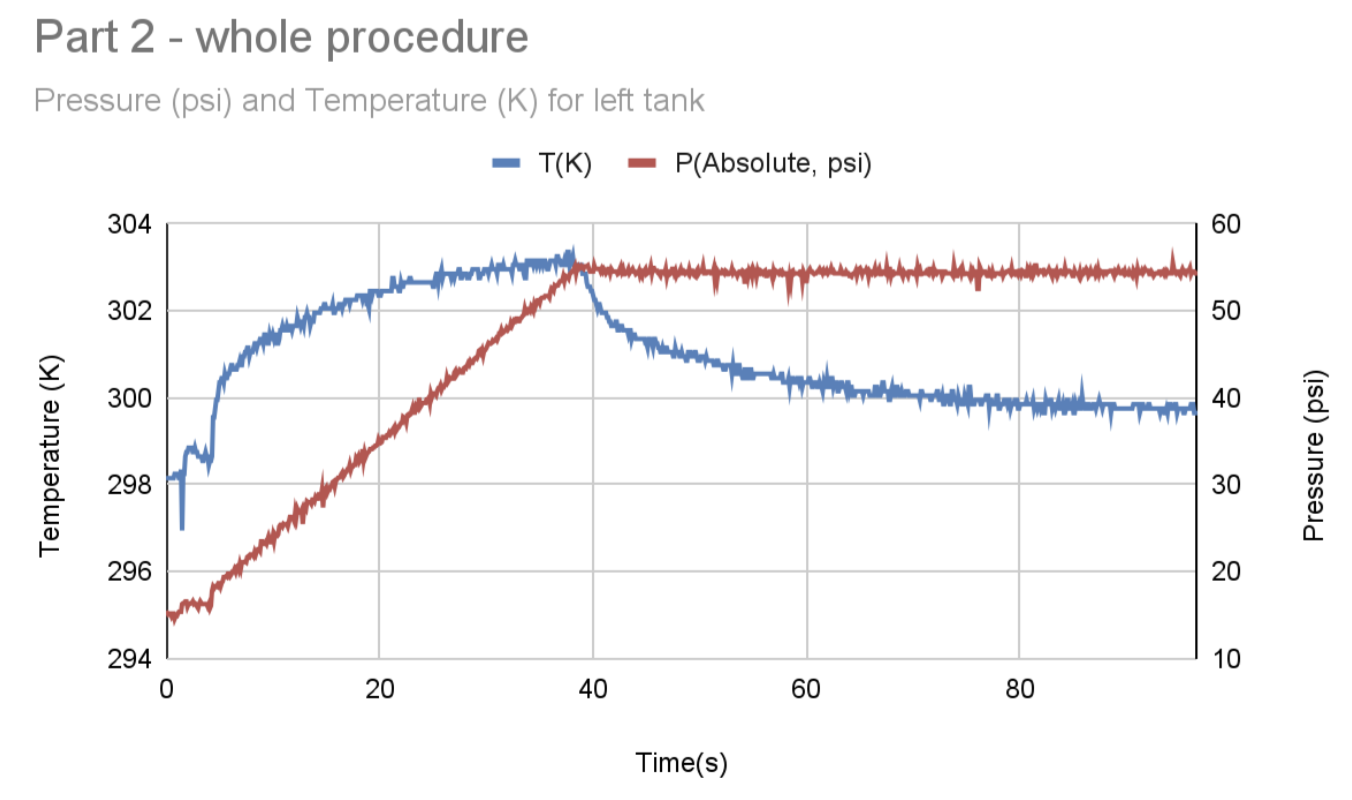
\includegraphics[width=0.48\columnwidth]{figure/p2.png}
        \label{fig:p2}
    }
    \hfill
    \subfloat[Mass Flow Rate]{
        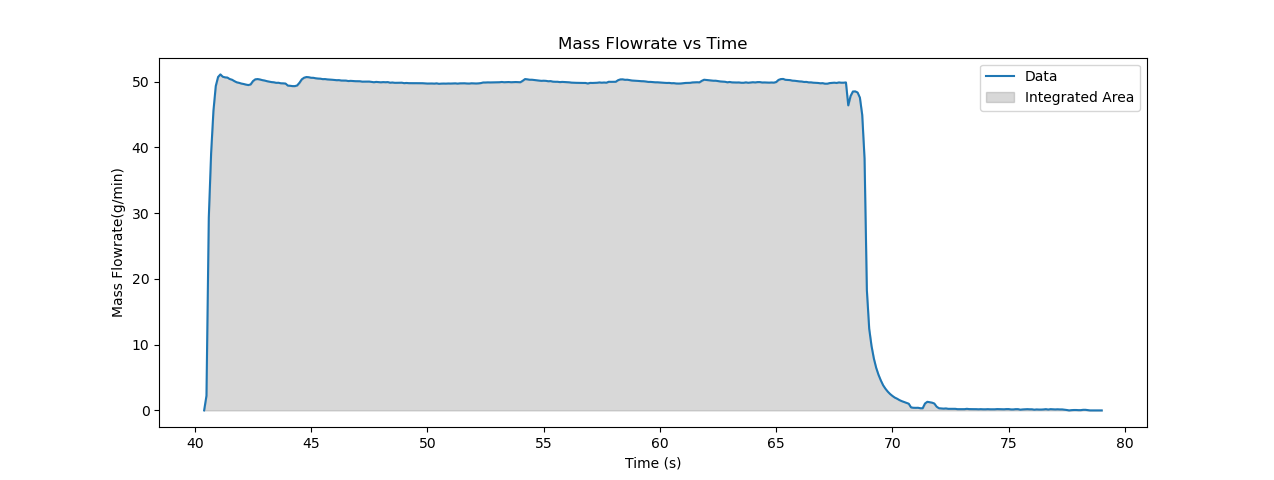
\includegraphics[width=0.45\columnwidth]{figure/mass.png}
        \label{fig:mass}
    }
    \caption{Plots of recorded data for experiment II.}
    \label{fig:graphs2}
\end{figure}
Upon pressurization and once the tank achieved thermal equilibrium, the absolute pressure within the tank stood at $54.3\pm0.3[psig]$, with the temperature registering $299.3\pm0.2[K]$ (Uncertainties determined visually) (Fig. \ref{fig:p2}). 
\subsubsection*{Discussion}
\begin{itemize}
    \item Identifying initial mass and volume:\\
    We recognized that to accurately identify the mass in the container at $40[psig]$,, $m_{40}$ both the initial mass of air under ambient pressure, $m_i$, and the mass added by pressurizing the tank, $\Delta m$, must be considered. $\Delta m$ could be computed by numerically integrating the mass flow rate curve, $\dot{m}$ (Fig. \ref{fig:mass}) using trapezoidal sums with $\Delta t=0.1$ being the time interval between data collection instances:
    \begin{equation}
        \Delta m = \int_{t_i}^{t_f}\dot{m}(t)dt = \sum_{i=1}^{410-1}\frac{\Delta t}{2}(\dot{m_i}+\dot{m}_{i+1})= 29.3 \pm 0.7 \; [g]
    \end{equation}
    Where uncertainty is computed by propagating the visually interpreted uncertainty $u(\dot{m})=0.2$.  And since the process is isochoric, the following must hold true:
    \begin{equation}
        \begin{cases}
            V = \frac{m_iRT_i}{P_i} \\
            V = \frac{m_{40}RT_{40}}{P_{40}}
        \end{cases}
    \end{equation}
    Equating them, we arrived at:
    \begin{align}
        \frac{m_iT_i}{P_i} &= \frac{(m_{i}+\Delta m )T_{40}}{P_{40}}
        % \frac{m_i\cdot298.2[k]}{16.1282[psi]} &= \frac{(m_{i}+30.1[g])\cdot 299.7[k]}{56.1282[psi]}\\
        % \implies m_i &= 12.2\pm0.5[g]\\
    \end{align}
    For which solving the equation gives $m_i = 12.2\pm0.5[g]$ after adjusting the pressure to psi by accounting for the ambient pressure. Summing the initial and the mass added to pressurize the vessel to $40 [psig]$, calculations yielded a total system mass, $m_i+\Delta m$ of $42.3\pm0.5[g]$. Then, values can be inputted into equation (7) to arrive at an initial volume of $8.48\pm0.01[L]$.
    % \begin{align}
    %     V=\frac{0.0122[kg]\cdot0.287\left[\frac{kJ}{kg\cdot k}\right]\cdot298.2[k]}{111[kPa]} &= \frac{(0.0485)[kg]\cdot0.287\left[\frac{kJ}{kg\cdot k}\right]\cdot299.7[k]}{387[kPa]}\\
    %     &=0.0108[m^3]=10.8\pm0.1[L]
    % \end{align}
    % Therefore, the initial mass of air in the tank under ambient pressure is $14.0\pm0.5[g]$ and the volume of the left tank is $10.8\pm0.1[L]$.
    \item In this experiment, numerous assumptions were made about the setup, yet not all of them were accurate and hence possible sources of errors must be considered:\\
    \begin{enumerate}
        \item The external environment's temperature was 1.3[K] lower than the initial temperature within the tank, indicating a temperature difference between the pressurized air and the tank's original air content. The difference may lead to errors in the calculation.
        \item The sensors measuring thermodynamic properties exhibited minor fluctuations, suggesting potential inaccuracies, even when the values were expected to remain constant.
        \item In the analysis, the gas has been treated as an ideal gas, however, there are still minute intermolecular forces present and molecules inevitably occupy some volume and thus our assumptions will introduce slight inaccuracies.
        \item In practical experiments, equipment errors are unavoidable. Potential leaks in the tank, tubes, and valves can introduce inaccuracies to the analysis.
    \end{enumerate}
    \item Compressibility of air \& its impact on results:\\
    The compressibility of gas measures how much a given quantity of it will decrease in volume when applied pressure \autocite{al-raeei2020formula}. It is denoted by:
    \begin{equation}
        Z=\frac{PV}{RT}
    \end{equation}
    For an ideal gas, where the minimal intermolecular forces and volumes occupied by molecules can be ignored, compressibility will always equal one since for a mole of gas, $PV=RT$. Hence we can conclude that the compressibility of air is irrelevant to our results.
    % However, in real gases, the relationship between state properties such as pressure, volume, and temperature is affected by compressibility, which could be proved by Boyle’s Law and Charles’s Law.
    % Boyle’s Law shows the relationship between pressure and volume, where at the same temperature, the volume is inversely proportional to pressure:
    % \begin{equation}
    %     P=\frac{c_2}{V}
    % \end{equation}
    % Furthermore, Charle’s Law demonstrates that pressure and temperature have a proportional relationship:
    % \begin{equation}
    %     V=c_3T
    % \end{equation}
    % This demonstrates that in a real gas, path-independent values such as pressure, volume, and temperature have interconnected relationships with compressibility.
\end{itemize}
\section*{Conclusion}
In conclusion, this experiment successfully demonstrated the path independence of thermodynamic state properties and determined their relationships under different conditions. Unknown values and properties such as initial volume, initial mass and volume ratios were determined using the Ideal Gas Law. While the results were generally in line with theoretical expectations, minor sources of error, such as temperature differences and sensor fluctuations, were noted. Overall, this experiment provided practical insights into thermodynamic phenomena and the behavior of gaseous systems.
% \newpage
\printbibliography
\end{document}